\documentclass[10pt]{article}
\usepackage[spanish,es-tabla]{babel}
\usepackage[left=2.5cm,bottom=4.5cm]{geometry}
\usepackage{amsmath,amssymb}
\spanishdecimal{.}
\usepackage[utf8]{inputenc}
\usepackage{graphicx}
\usepackage{hyperref} % Para que las ecuaciones referencíen con links
\usepackage{booktabs}
\usepackage{fullpage}
\usepackage{float}
\usepackage{lscape}
\usepackage{parskip}
\setlength{\parindent}{0pt}
\title{Práctica 2 Procesos Estocásticos MCMC}
\date{\today}
\author{Fernando Avitúa Varela}
\begin{document}
\maketitle

En esta práctica se trabajarán los conceptos aprendidos en la primera parte del curso acerca de cadenas de Markov. Revisaremos el tema de Monte Carlo Markov Chain (MCMC por sus siglas en inglés). La primera parte de este título, \emph{Monte Carlo}, trata de  cómo hacer simulaciones para realizar algún cálculo que puede ser desde una estimación puntual hasta obtener intervalos de confianza. Este método es usado con cadenas de Markov para realizar simulaciones de distribuciones que normalmente son muy complicadas. En esta práctica, veremos un pequeño ejemplo de las dos partes.

\section*{Monte Carlo: Aceptación Rechazo}

El método de aceptación-rechazo (que revisaremos en clase) es usado para simular de distribuciones continuas y acotadas (existe también un método para distribuciones no acotadas). Para llevarlo acabo primero se realiza una simulación en un cuadrado que encierre a la distribución que estamos intentando simular. Después, dentro de este cuadrado simularemos de manera uniforme puntos tal que etiquetaremos a los que caen por debajo de la función de distribución como aceptados y al resto como rechazados (Figura 1).


Dentro de los puntos aceptados tomamos sus coordenadas $x$ y estos forman una simulación de la variable aleatoria de interés como podemos ver en la Figura 2.


\begin{figure}[H]
    \centering
    \begin{minipage}[b]{0.45\textwidth}  % Adjust the width to fit your document
        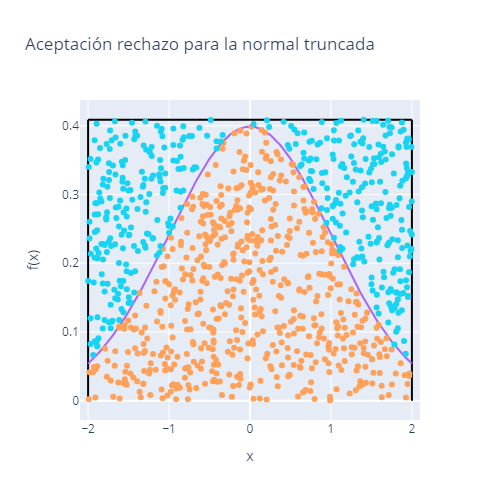
\includegraphics[scale=.3]{ar.png}
        \caption{Diagrama usado para simular de la distribución normal}
        \label{fig:ar}
    
    \end{minipage}
    \hfill  % Adds horizontal space between the two minipages
    \begin{minipage}[b]{0.45\textwidth}  % Adjust the width to fit your document
        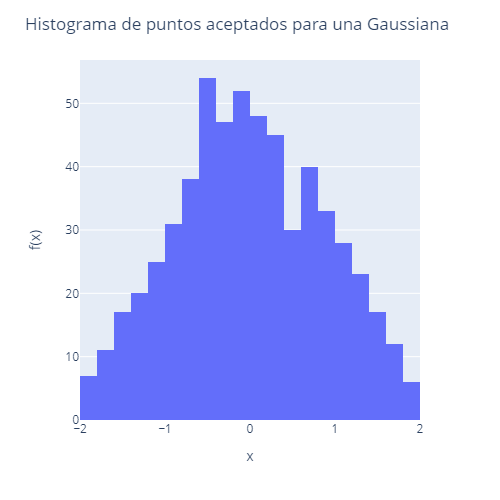
\includegraphics[scale=.3]{hist.png}
        \caption{Histograma de puntos obtenidos al hacer una proyección}
        \label{fig:hist}
  
    \end{minipage}
\end{figure}

\begin{enumerate}
    \item 
    \framebox{\parbox{\dimexpr\linewidth-2\fboxsep-2\fboxrule}{\itshape%,
    Usa el método de aceptación rechazo para generar 10 mil simulaciones de alguna distribución de tu elección (puede ser discreta o continua), después la tendrás que generar también usando MCMC.
    }}


\section*{Markov Chain: Metropolis-Hastings}

El objetivo será diseñar un juego que tiene 4 estados como los mostrados en la Figura 3. Como vimos en clase, tenemos que para cada estado tendremos una recompensa diferente antes de dar un paso al siguiente estado.  
\begin{figure}[H]
    \centering
    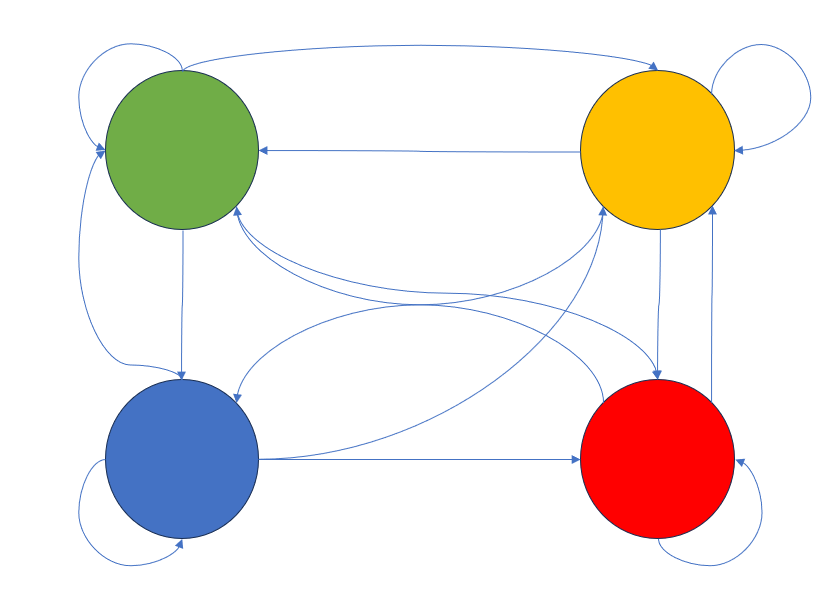
\includegraphics[scale=0.5]{tablero.png}
    \caption{Juego visto en clase. Cada nodo es un estado del juego y las flechas representan las transiciones (pueden ser cero).}
    \label{fig:juego}
\end{figure}

\item 
\framebox{\parbox{\dimexpr\linewidth-2\fboxsep-2\fboxrule}{\itshape%,
Propón una matriz de transición entre los estados y después describe las clases de comunicación de la cadena ¿Por qué podemos asegurar que tiene una distribución estacionaria?

Encuentra la distribución estacionaria de la distribución anterior ya sea simulando o sin hacerlo. 

Encuentra una función de recompensa para cada estado que hace al juego justo.
}}


En esta parte haremos lo contrario al ejercicio anterior: Ahora tenemos una distribución estacionaria y queremos encontrar la función de transición entre los estados que nos dé esa distribución estacionaria.

Supón que la función de recomensa está dada por $$ R=(R_{\text{verde}},R_{\text{amarillo}},R_{\text{azul}},R_{\text{rojo}})=(100,-500,25,1) $$

\item 
\framebox{\parbox{\dimexpr\linewidth-2\fboxsep-2\fboxrule}{\itshape%,
Encuentra la distribución estacionaria que dada la previa función de recompensa nos da un juego justo. Después usa el método de Metropolis-Hastings para obtener la matriz de transición del juego. 
}}

\item
\framebox{\parbox{\dimexpr\linewidth-2\fboxsep-2\fboxrule}{\itshape%,
Por último usa el método de Metropolis-Hastings para hacer una simulación de la distribución que escogiste en la primer pregunta. Compara los histogramas, revisa el tiempo que toma cada uno y discute acerca del periodo de quemado de la cadena.
}}

\end{enumerate}


\end{document}